\documentclass[12pt, twoside]{article}
\usepackage[letterpaper, margin=1in, headsep=0.5in]{geometry}
\usepackage[english]{babel}
\usepackage[utf8]{inputenc}
\usepackage{amsmath}
\usepackage{amsfonts}
\usepackage{amssymb}
\usepackage{tikz}
\usetikzlibrary{quotes, angles}
\usepackage{graphicx}
\usepackage{enumitem}
\usepackage{multicol}

\newif\ifmeta
\metatrue %print standards and topics tags

\title{Regents Geometry}
\author{Chris Huson}
\date{September 2020}

\usepackage{fancyhdr}
\pagestyle{fancy}
\fancyhf{}
\renewcommand{\headrulewidth}{0pt} % disable the underline of the header
\raggedbottom


\fancyhead[LE]{\thepage}
\fancyhead[RO]{\thepage \\ Name: \hspace{4cm} \,\\}
\fancyhead[LO]{BECA / Dr. Huson / Geometry 07-Similarity\\* pset ID: 108}

\begin{document}

\subsubsection*{7-3bDN-Tangent}
\begin{enumerate}
\item \begin{enumerate}
    \item Graph and label $\triangle ABC$ with $A(0,0)$, $B(7,4)$, and $C(7,0)$.
    \begin{center}
      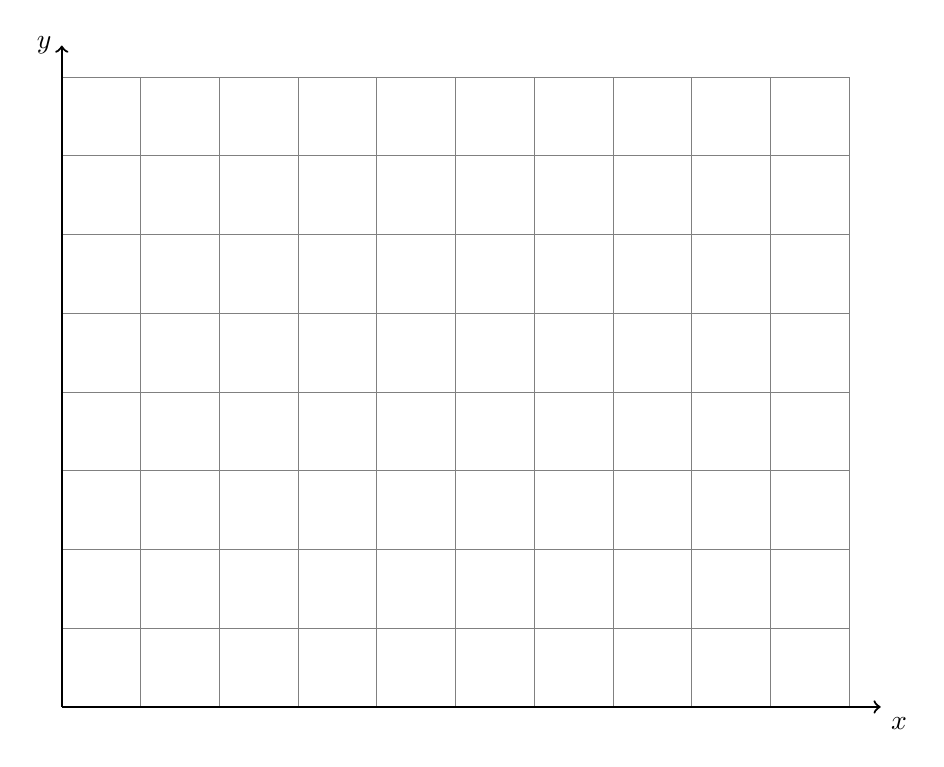
\begin{tikzpicture}
        \draw [help lines] (0,0) grid (10,8);
        \draw [thick, ->] (0,0) -- (10.4,0) node [below right] {$x$};
        \draw [thick, ->] (0,0)--(0,8.4) node [left] {$y$};
      \end{tikzpicture}
    \end{center}
    \item Find the lengths of the sides of $\triangle ABC$.
    \begin{multicols}{2}
      $AC=$ \hspace{3cm}
      $BC=$ \\[1cm]
      $AB=\sqrt{AC^2+BC^2}$
    \end{multicols} \vspace{2.5cm}
    \item Find the slope and $y$-intercept of the line $\overleftrightarrow{AB}$.
      \begin{multicols}{2}
        $m_{AB}=$ \\
        $b_{AB}=$
      \end{multicols} \vspace{0.5cm}
    \item Write down the equation of each line. \\[0.5cm]
      $\overleftrightarrow{AB}$: \hfill
      $\overleftrightarrow{BC}$: \hfill
      $\overleftrightarrow{AC}$: \hspace{2cm}
    \vspace{2cm}
    \item Find the measure of $\angle BAC$ in degrees with a protractor.
  \end{enumerate}


\end{enumerate}
\end{document}